\documentclass[a4paper,12pt]{article}
\usepackage[utf8]{inputenc}
\usepackage[T1]{fontenc}

\usepackage[francais]{babel}

\usepackage{algorithmeUTF8}
\usepackage{listings}
\lstset{breaklines=true}
\usepackage{verbatim}
\usepackage{graphicx}
\usepackage{listings}
\usepackage{xcolor}
\lstset { %
	language=C++,
	backgroundcolor=\color{black!5}, % set backgroundcolor
	basicstyle=\footnotesize,% basic font setting
}
\title{Projet d'Algorithmique avancée\\ \huge Othello}
\author{\textbf{Groupe 1.3}\\KLEIBER Lise\\IMBERT Gauthier\\SERSOURI Mohamed\\DAVID Maxence}
\date{\today}

\begin{document}
\maketitle
\newpage
\tableofcontents
\newpage
\section{Introduction}
Le jeu d'othello est un jeu de stratégie qui se joue à deux joueurs, un joueur blanc et un joueur noir. 
Ce jeu se joue en principe sur un plateau appelé othellier, ce plateau est composé de 64 cases (8 \times 8).
Le but est simple : avoir le plus de pion de sa couleur a la fin de la partie.\\
Pour cela chaque joueur peut capturer les pion adverse en les encerclant par des pion de sa couleur. 
 Le but de notre projet d'algoritmique est de réaliser un  un programme informatique permetant de jouer a l'Othello sur sa machine.
Pour cela il nous faudra réaliser la specification des TAD indispendable pour notre futur programme. Puis réaliser la conception préliminaire ainsi que la conception detaillée du problème.
Dans un second temps nous devront implémenter notre solution en utilisant le language de programmation spécifique au cours : le C. 
Pour finir nous devront mettre en place une batterie de tests unitaires pour nous assurer du bon fonctionnement de chaque fonctionnalité implentée.\\
De plus il nous est demandé de réaliser une Intelligence artificielle dans le but de pouvoir jouer contre l'ordinateur.\\
Mais aussi de confronter notre algoritme avec celui des autres groupe à l'occasion d'un tournoi.
Ce projet est une première approche de projet de groupe pour réaliser un programme informatque, avec tout ce qui est impliqué par la création d'un programme du debut a la fin.
Avec nottament la prise de decisions sur des choix d'implementation. Mais aussi la gestion du code grâce à GIT.  
 Ce projet va  aussi nous permettre  de nous amméliorer dans la programmation en C.
 


\newpage
\documentclass{article}
\usepackage{algorithmeUTF8}

\begin{document}

  \section{TAD}
    \subsection{Couleur}
    \begin{tad}
        \tadNom{Couleur}
        %\tadParametres{Element,Clef}
        %\tadDependances{\booleen}
        \begin{tadOperations}{Couleur}
            \tadOperation{Blanc}{}{\tadUnParam{Couleur}}
            \tadOperation{Noir}{}{\tadUnParam{Couleur}}
            \tadOperation{ChangerCouleur}{\tadUnParam{Couleur}}{\tadUnParam{Couleur}}
        \end{tadOperations}
        % \begin{tadSemantiques}{Couleur}
        %     \tadSemantique{dictionnaire}{l’op´eration qui permet de construire un Couleur `a partir de sa partie r´eelle et imaginaire}
        %     \tadSemantique{ajouter}{L’op´eration qui permet d’ajouter un ´el´ement dans le Couleur}
        %     \tadSemantique{retirer}{L’op´eration qui permet de retirer un ´element du Couleur}
        % \end{tadSemantiques}
        \begin{tadAxiomes}
            \tadAxiome{ChangeC(Blanc)=Noir}
            \tadAxiome{ChangeC(Noir)=Blanc}
        \end{tadAxiomes}
    \end{tad}
    \subsection{Pion}
    \begin{tad}
        \tadNom{Pion}
        %\tadParametres{Element,Clef}
        \tadDependances{Couleur, Coup}
        \begin{tadOperations}{Pion}
            \tadOperation{CreerPion}{\tadUnParam{Couleur}}{\tadUnParam{Pion}}
            \tadOperation{FlipPion}{\tadUnParam{Pion}}{\tadUnParam{Pion}}
            \tadOperation{ObtenirCouleurPion}{\tadUnParam{Pion}}{\tadUnParam{Couleur}}
        \end{tadOperations}
        % \begin{tadSemantiques}{Couleur}
        %     \tadSemantique{dictionnaire}{l’op´eration qui permet de construire un Couleur `a partir de sa partie r´eelle et imaginaire}
        %     \tadSemantique{ajouter}{L’op´eration qui permet d’ajouter un ´el´ement dans le Couleur}
        %     \tadSemantique{retirer}{L’op´eration qui permet de retirer un ´element du Couleur}
        % \end{tadSemantiques}
        \begin{tadAxiomes}
            \tadAxiome{ObtenirCouleurPion(Pion(a))=a}
            \tadAxiome{FlipPion(FlipPion(a))=a}
        \end{tadAxiomes}
    \end{tad}
    \subsection{Position}
    \begin{tad}
        \tadNom{Position}
        %\tadParametres{Element,Clef}
        \tadDependances{\caractere, \booleen}
        \begin{tadOperations}{Position}
            \tadOperation{DefPosition}{\tadDeuxParams{\caractere}{\caractere}}{\tadUnParam{Position}}
            \tadOperation{Obtenirx}{\tadUnParam{Position}}{\tadUnParam{\caractere}}
            \tadOperation{Obteniry}{\tadUnParam{Position}}{\tadUnParam{\caractere}}
            \tadOperation{EstValide}{\tadDeuxParams{\caractere}{}\caractere}{\tadUnParam{Booleen}}
        \end{tadOperations}
        % \begin{tadSemantiques}{Couleur}
        %     \tadSemantique{dictionnaire}{l’op´eration qui permet de construire un Couleur `a partir de sa partie r´eelle et imaginaire}
        %     \tadSemantique{ajouter}{L’op´eration qui permet d’ajouter un ´el´ement dans le Couleur}
        %     \tadSemantique{retirer}{L’op´eration qui permet de retirer un ´element du Couleur}
        % \end{tadSemantiques}
        \begin{tadAxiomes}
            \tadAxiome{Obtenirx(DefPosition(x,y))=x}
            \tadAxiome{Obteniry(DefPosition(x,y))=y}
        \end{tadAxiomes}
   	\begin{tadPreconditions}/\tadPrecondition{DefPosition(car,car)}{EstValide(car, car)}
   	\end{tadPreconditions}
    \end{tad}
    \subsection{Coup}
    \begin{tad}
        \tadNom{Coup}
        %\tadParametres{Element,Clef}
        \tadDependances{\booleen,Pion,Position, Plateau, Couleur}
        \begin{tadOperations}{Coup}
            \tadOperation{PlacerCoup}{\tadTroisParams{Pion}{Plateau}{Position}}{\tadUnParam{Coup}}
            \tadOperation{ObtenirPosCoup}{\tadUnParam{Coup}}{\tadUnParam{Position}}
            \tadOperation{ObtenirCouleurCoup}{\tadUnParam{Coup}}{\tadUnParam{Couleur}}
            \tadOperation{CoupValide}{\tadTroisParams{Pion}{Plateau}{Position}}{\tadUnParam{\booleen}}
        \end{tadOperations}
        % \begin{tadSemantiques}{Couleur}
        %     \tadSemantique{dictionnaire}{l’op´eration qui permet de construire un Couleur `a partir de sa partie r´eelle et imaginaire}
        %     \tadSemantique{ajouter}{L’op´eration qui permet d’ajouter un ´el´ement dans le Couleur}
        %     \tadSemantique{retirer}{L’op´eration qui permet de retirer un ´element du Couleur}
        % \end{tadSemantiques}
        \begin{tadAxiomes}
            \tadAxiome{ObtenirPosCoup(PlacerCoup(p,pl,ps))=ps}
            \tadAxiome{ObtenirCouleurCoup(PlacerCoup(p,pl,ps))=p} %à revoir placerCoup(p,ps)=obtenirCpion(p)
        \end{tadAxiomes}
   	\begin{tadPreconditions}/\tadPrecondition{PlacerCoup(p, pl, ps) : CoupValide(p, pl, ps)}
   	\end{tadPreconditions}
   	        \end{tad}
    \subsection{Plateau}
    \begin{tad}
        \tadNom{Plateau}
        %\tadParametres{Element,Clef}
        \tadDependances{\booleen,Pion,Position, Coup}
        \begin{tadOperations}{Plateau}
            \tadOperation{CreerPlateau}{}{\tadUnParam{Plateau}}
            %\tadOperation{PoserPion}{\tadTroisParams{}}{\tadUnParam{Position}}
            \tadOperation{ObtenirPion}{\tadDeuxParams{Position}{Plateau}}{\tadUnParam{Pion}}
            \tadOperation{RetournerPion}{\tadTroisParams{Position}{Plateau}{Coup}}{\tadUnParam{Plateau}}
            \tadOperation{EstVide}{\tadDeuxParams{Position}{Plateau}}{\tadUnParam{\booleen}}
            \tadOperation{ViderPlateau}{\tadUnParam{Plateau}}{\tadUnParam{Plateau}}
            \tadOperation{EstGagnant}{\tadDeuxParams{Coup}{Plateau}}{\tadUnParam{\booleen}}
        \end{tadOperations}
    
   	\begin{tadPreconditions}/\tadPrecondition{ObtenirPion(ps, pl) : 	non(EstVide(pl))}\tadPrecondition{RetournerPion(ps, pl, c) : non(EstVide(pl))}
   		\tadPrecondition{ViderPlateau(pl) : non(estVide(pl))}
   		\tadPrecondition{EstGagnant(pl) : non(estVide(pl))}
\end{tadPreconditions}
    \end{tad}
    \subsection{Coups}
\begin{tad}
	\tadNom{Coups}
	\tadDependances{\naturel, \naturelNonNul, Coup, \booleen}
	\begin{tadOperations}{Coups}
		\tadOperation{InitCoups}{}{\tadUnParam{Coups}}
		\tadOperation{EstVide}{\tadUnParam{Coups}}{\tadUnParam{\booleen}}
		\tadOperation{AjouterCoup}{\tadDeuxParams{Coups}{Coup}}{\tadUnParam{Coups}}
		\tadOperation{IemeCoup}{\tadDeuxParams{Coups}{\naturelNonNul}}{\tadUnParam{Coup}}
		\tadOperation{NbCoups}{\tadUnParam{Coups}}{\tadUnParam{\naturel}}
		\tadOperation{EstPresent}{\tadUnParam{Coups}}{\tadUnParam{\naturel}}
	\end{tadOperations}
\begin{tadAxiomes}
	\tadAxiome{estVide(InitCoups())}
	\tadAxiome{nbCoups(InitCoups()) = 0}
	\tadAxiome {ajouter(cs,c) = nbCoups(cs)+1}
\end{tadAxiomes}
\begin{tadPreconditions}/\tadPrecondition{IemeCoup(c,i): i $\leq$ nbCoups(c)}
		\end{tadPreconditions}
\end{tad}
\end{document}
\newpage

\section{Signatures}
	\subsection{affichagePlateau}
		\begin{algorithme}
			\signatureprocedure
				{affichagePlateau}
				{\paramEntree{pl : Plateau}}
		\end{algorithme}
	\subsection{creerPlateau}
		\begin{algorithme}
			\signaturefonction
				{creerPlateau}
				{}
				{Plateau}
		\end{algorithme}
	\subsection{majPlateau}
		\begin{algorithme}
			\signaturefonction
				{majPlateau}
				{lePlateau : Plateau, leCoup : Coup}
				{Plateau}
		\end{algorithme}
	\subsection{testLignes}
		\begin{algorithme}
			\signaturefonction
				{testLignes}
				{laPosition : Position}
				{Position, Booleen}
		\end{algorithme}
	\subsection{testColonnes}
		\begin{algorithme}
			\signaturefonction
				{testColonnes}
				{laPosition : Position}
				{Position, Booleen}
		\end{algorithme}
	\subsection{testDiagonales}
		\begin{algorithme}
			\signaturefonction
				{testDiagonales}
				{laPosition : Position}
				{Position, Booleen}
		\end{algorithme}
	\subsection{retournerPion}
		\begin{algorithme}
			\signatureprocedure
				{retournerPion}
				{p : Pion, lePlateau : Plateau, laPosition : Position}
		\end{algorithme}
	\subsection{changerCouleur}
		\begin{algorithme}
			\signaturefonction
				{changerCouleur}
				{laCouleur : Couleur}
				{Couleur}
		\end{algorithme}

	\subsection{placerCoup}
		\begin{algorithme}
			\signaturefonction
				{placerCoup}
				{lePion : Pion,laPosition : Position, lePlateau : Plateau}
				{Coup}
		\end{algorithme}
	\subsection{definirCouleurNouveauJoueur}
		\begin{algorithme}
			\signaturefonction
				{definirCouleurNouveauJoueur}
				{dernierPionPlace : Pion}
				{Couleur}
		\end{algorithme}
	\subsection{definirPosition}
		\begin{algorithme}
			\signaturefonction
				{definirPosition}
				{abcisse, ordonnee : \caractere}
				{Postition}
		\end{algorithme}
	\subsection{coupValide}
		\begin{algorithme}
			\signaturefonction
				{coupValide}
				{lePion : Pion, positionCoup : Position, lePlateau : Plateau}
				{\booleen}
		\end{algorithme}
	\subsection{estVide}
		\begin{algorithme}
			\signaturefonction
				{estVide}
				{pl : Plateau, positionCoup : Position}
				{\booleen}
		\end{algorithme}
	\subsection{retournerAuMoinsUnPion}
		\begin{algorithme}
			\signaturefonction
				{retournerAuMoinsUnPion}
				{pl : Plateau, leCoup : Coup}
				{\booleen}
		\end{algorithme}
	\subsection{partieTerminee}
		\begin{algorithme}
			\signaturefonction
				{partieTerminee}
				{pl : Plateau}
				{\booleen}
		\end{algorithme}
	\subsection{plateauPlein}
		\begin{algorithme}
			\signaturefonction
				{plateauPlein}
				{lePlateau : Plateau}
				{\booleen}
		\end{algorithme}
	\subsection{estGagnant}
		\begin{algorithme}
			\signaturefonction
				{estGagnant}
				{pl : Plateau, lePion : Pion}
				{\booleen, Couleur}
		\end{algorithme}
	\subsection{obtenirCouleur}
		\begin{algorithme}
			\signaturefonction
				{obtenirCouleur}
				{p : Pion}
				{Couleur}
		\end{algorithme}
	\subsection{plusDeCoups}
		\begin{algorithme}
			\signaturefonction
				{plusDeCoups}
				{pl : Plateau}
				{\booleen}
		\end{algorithme}
	\subsection{faireUnePartie}
\begin{algorithme}
	\signaturefonction
	{faireUnePartie}
	{}
	{Couleur}
\end{algorithme}
	\subsection{moduleIA}
\begin{algorithme}
	\signaturefonction
	{moduleIA}
	{pl : Plateau}
	{Coup}
\end{algorithme}
	\subsection{scoreDUnCoup}
\begin{algorithme}
	\signaturefonction
	{scoreDUnCoup}
	{lesCoups : Coups}
	{\naturel}
\end{algorithme}
	\subsection{minMax}
\begin{algorithme}
	\signaturefonction
	{minMax}
	{lesCoups : Coups}
	{Coup}
\end{algorithme}

	\subsection{evaluer}
\begin{algorithme}
	\signaturefonction
	{evaluer}
	{leCoupAEvaluer : Coup}
	{\naturel}
\end{algorithme}

	\subsection{coupsPossibles}
\begin{algorithme}
	\signaturefonction
	{coupsPossibles}
	{lePlateau : plateau}
	{Coups}
\end{algorithme}

	\subsection{nbCoups}
\begin{algorithme}
	\signaturefonction
	{nbCoups}
	{lesCoups : Coups}
	{\naturel}
\end{algorithme}

	\subsection{iemeCoup}
\begin{algorithme}
	\signaturefonction
	{iemeCoup}
	{lesCoups : Coups, indice : \naturelNonNul}
	{Coup}
\end{algorithme}

\newpage

\section{Conception détaillée}
\subsection{TAD}
\subsubsection{Couleur}
\begin{algorithme}

	\fonction 
	{Blanc}
	{}
	{Couleur}
	{}
	{\retourner{Blanc}}
	\fonction 
	{Noir}
	{}
	{Couleur}
	{}
	{\retourner{Noir}}
	\fonction
	{changerCouleur}
	{couleurActuelle : Couleur}
	{Couleur}
	{}
	{
		\sialorssinon{couleurActuelle = Blanc}{
			\retourner{Noir}
		}
			{
				\retourner{Blanc}
			}
			
	}
	\fonction
	{estBlanc}
	{uneCouleur : Couleur}
	{\booleen}
	{}
	{\sialorssinon{uneCouleur = Noir}
		{\retourner{1}
	}
{\retourner{0}
}
}
	\fonction
	{estNoir}
	{uneCouleur : Couleur}
	{\booleen}
	{}
	{\sialorssinon{uneCouleur = Blanc}
		{\retourner{1}
		}
		{\retourner{0}
	}}

\end{algorithme}

\subsubsection{Coup}
\begin{algorithme}
	\fonction 
	{initCoup}
	{position : Position, pion : Pion}
	{Coup}
	{leCoup : Coup}
	{\affecter{leCoup.positionCoup}{position}
	\affecter{leCoup.Pion}{pion}
	\retourner{leCoup}
	}

	
	\fonction 
	{obtenirPositionCoup}
	{coup : Coup}
	{Position}
	{}
	{\retourner{coup.positionCoup}}
	
	\fonction 
	{obtenirPionCoup}
	{coup : Coup}
	{Pion}
	{}
	{\retourner{coup.Pion}}
	
	\fonction 
	{obtenirCouleurCoup}
	{coup : Coup}
	{Couleur}
	{}
	{\retourner{obtenirCouleurPion(coup.Pion)}}
	
	
	\fonction 
{coupValide}
{leCoup : Coup, lePlateau : Plateau}
{\booleen}
{position : Position}
{
	\affecter{position}{leCoup.positionCoup}
	\retourner{(lePlateau[obtenirX(position)-1][obtenirY(position)-1].etatPion = 0) ET retournerAuMoinsUnPion(lePlateau,leCoup)}
	
}


\fonction 
{obtenirPionCoup}
{coup1, coup2 : Coup}
{\booleen}
{}
{
	\retourner{egal(coup1.Pion,coup2.Pion) ET egal(coup1.positionCoup,coup2.positionCoup)}
}

\end{algorithme}
\subsubsection{Coups}
\begin{algorithme}
\fonction
{initCoups}
{}
{Coups}
{coups : Coups}
{\affecter{coups.nbCoups}{0}
\retourner{coups}}

\fonction
{estVide}
{coups : Coups}
{\booleen}
{}
{\retourner{coups.nbCoups = O} }

\fonctionAvecPreconditions
{iemeCoup}
{coups : Coups, i : \naturel}
{Coup}
{i $>$0 ET i $<= $ nbCoups(coups)}
{}
{\retourner{coups.tabCoups[i-1]} }

\procedureAvecPreconditions
{ajouterCoup}
{{\paramEntreeSortie{coups : Coups, }}{\paramEntree{coup : Coup}}}
{nbCoups(coups) $<$ MAX}{}
{\affecter{tabcoups[nbCoups(coups)]}{coup}
\affecter{nbCoups}{nbCoups+1}}


\fonction
{nbCoups}
{coups : Coups}
{\naturel}
{}
{\retourner{coups.nbCoups}}

\fonctionAvecPreconditions
{estPresent}
{coups : Coups, coup : Coup}
{\booleen}
{non(estVide(coups))}
{i : \naturelNonNul, test = \naturel}
{\pour{i}{1}{coups.nbCoups}{}{
		\sialors{obtenirX(obtenirPositionCoup(coups.tabcoups[i])) = obtenirX(obtenirPositionCoup(coup)) ET obtenirY(obtenirPositionCoup(coups.tabcoups[i])) = obtenirY(obtenirPositionCoup(coup) ET obtenirCouleurCoup(coups.tabcoups[i]) = obtenirCouleurCoup(coup) = 1}{
			\affecter{test}{1}
		}
}
\retourner{test}
}
	
\procedure
{supprimerCoup}
{\paramEntreeSortie{coups : Coups, }{\paramEntree{i : \naturel}}}
{j : \naturel}
{
	\affecter{j}{0}	
	\pour{j}{i}{nbCoups-1}{}{
		\affecter{tabCoups[i]}{tabCoups[i+1]}
	}
\affecter{nbCoups}{nbCoups-1}
}

\fonction
{obtenirCoupsPossible}
{pl : Plateau, couleurReference : Couleur}
{Coups}
{j,i : \naturel, pion : Pion, position : Position, resultat : Coups}
{
		\affecter{j}{0}
		\affecter{i}{0}
		\affecter{resultat}{initCoups()}
		\affecter{pion}{creerPion(CouleurReference)}
	\pour{i}{1}{8}{}{
		\pour{j}{1}{8}{}{
				\affecter{position}{defPosition(i,j)}
					\affecter{coup}{initCoup(position, pion)}
					\sialors{coupValide(coup, pl)}{
						\instruction{ajouterCoup(resultat, coup)}
					
				}
	
}
	
}
\retourner{resultat}
}


\end{algorithme}

\subsubsection{Pion}
\begin{algorithme}

\fonction
{creerPion}
{couleur : Couleur}
{Pion}
{resultat : Pion}
{\affecter{resultat.couleurPion}{couleur}
\affecter{resultata.etatPion}{1}
\retourner{resultat}}

\procedure
{changerEtat}
{\paramEntreeSortie{pion : Pion}}
{resultat : Pion}
{\sialorssinon{pion.etatPion =0}
{\affecter{resultat.etatPion}{1}
}
{\affecter{resultat.etatPion}{0}
}
}
\fonction
{obtenirCouleurPion}
{pion : Pion}
{Couleur}
{}
{\retourner{pion.couleurPion}}

\fonction
{obtenirEtatPion}
{pion : Pion}
{\naturel}
{}
{\retourner{pion.etatPion}}

\fonction
{egal}
{pion1, pion2 : Pion}
{\booleen}
{}
{\retourner{obtenirCouleurPion(pion1) = obtenirCouleurPion(pion2)}}
\end{algorithme}

\subsubsection{Plateau}
\begin{algorithme}

\procedure
{quatrePionsDebut}
{\paramEntreeSortie{plateau : Plateau}}
{}
{\instruction initialiserPlateau(plateau)
	
\instruction	poserPion(creerPion(Blanc()), \instruction defPosition(4,4), plateau)
\instruction	poserPion(creerPion(Noir()), \instruction defPosition(4,5), plateau)
\instruction	poserPion(creerPion(Blanc()), \instruction defPosition(5,5), plateau)
\instruction	poserPion(creerPion(Noir()), \instruction defPosition(5,4), plateau)}

\procedure
{initialiserPlateau}
{\paramEntreeSortie{plateau : Plateau}}
{i, j : \naturelNonNul, position : Position}
{\pour{i}{1}{HAUTEUR}{}{
		\pour{j}{1}{LARGEUR}{}{
			\affecter{position}{defPosition(i,j)}
			\affecter{plateau)[obtenirX(position)-1][obtenirY(position)-1].etatPion}{0}
			}
}}

\fonction
{obtenirPion}
{position : Position, plateau : Plateau}
{Pion}
{}
{\retourner{plateau[obtenirX(position)-1][obtenirY(position)-1]}}

\procedureAvecPreconditions
{poserPion}
{\paramEntreeSortie{{plateau : Plateau, }}{\paramEntree{pion : Pion, position : Position}}}
{estVide(position,plateau)}
{}
{\affecter{plateau)[obtenirX(position)-1][obtenirY(position)-1]}{pion}}

\fonction
{estVide}
{position : Position, plateau : Plateau}
{\booleen}
{}
{\sialorssinon{obtenirEtatPion(obtenirPion(position,plateau)) = 0}{
		\retourner{1}
}
{		\retourner{0}
}
}

\procedure
{copierPlateau}
{\paramEntreeSortie{{plateau : Plateau, }}{\paramEntree{plateauACopier : Plateau}}}
{i, j : \naturelNonNul, position : Position, pion : Pion }
{\pour{i}{1}{HAUTEUR}{}{
		\pour{j}{1}{LARGEUR}{}{
			\affecter{position}{defPosition(i,j)}
			\affecter{plateau)[obtenirX(position)-1][obtenirY(position)-1].etatPion}{0}
			\affecter{pion}{obtenirPion(position, plateauACopier)}
			\sialors{non(estVide(position,plateauACopier))}{
				\instruction{poserPion(pion,position,plateau)}
			}
	}}
}

\end{algorithme}

\subsubsection{Position}
\begin{algorithme}
\fonction
{defPosition}
{x,y : \caractere}
{Position}
{resultat : Position}
{\affecter{resultat.positionx}{x}
\affecter{resultat.positiony}{y}
\retourner{resultat}
}


\fonction
{obtenirX}
{position : Position}
{\caractere}
{}
{\retourner{position.positionx}}

\fonction
{obtenirY}
{position : Position}
{\caractere}
{}
{\retourner{position.positiony}}

\fonction
{egal}
{pos1, pos2 : Position}
{\booleen}
{}
{\retourner{obtenirX(pos1) = obtenirX(pos2) ET (obtenirY(pos1) = obtenirY(pos2)}}
\end{algorithme}
       

        \subsection{obtenirCouleurGagnant}
        \begin{algorithme}
            \fonction
                {obtenirCouleurGagnant}
                {pl : Plateau}
                {\booleen , Couleur}
                {nbPionsNoirs, nbPionsBlancs, i, j : \naturel}
                {
                    \affecter{nbPionsNoirs}{0}
                    \affecter{nbPionsBlancs}{0}
                    \pour{i}{1}{8}{}
                    {
                        \pour{j}{1}{8}{}
                        {
                            \sialorssinon{obtenirCouleur(obtenirPion(defPosition(i,j),pl))=Noir}
                            {
                                \affecter{nbPionsNoirs}{nbPionsNoirs+1}   
                            }
                            {
                                \sialors{obtenirCouleur(obtenirPion(defPosition(i,j),pl))=Blanc}
                                {
                                    \affecter{nbPionsBlancs}{nbPionsBlancs+1}
                                }
                            }
                        }
                    }
                    \sialorssinon{nbPionsNoirs $>$ nbPionsBlancs}
                    {
                        \retourner{FAUX , Noir}
                    }
                    {
                        \sialorssinon{nbPionsNoirs $<$ nbPionsBlancs}
                        {
                            \retourner{FAUX , Blanc}
                        }
                        {
                            \retourner{VRAI , Blanc} $on retourne VRAI si egalite et une couleur par defaut$
                        }
                    }
                }
        \end{algorithme}

    \subsection{plusDeCoups}
        \begin{algorithme}
            \fonction
                {plusDeCoups}
                {pl : Plateau, couleurJoueurCourant : Couleur}
                {\booleen}
                {i, j : \naturelNonNul \\ coupOK : \booleen}
                {
                    \affecter{coupOK}{FAUX}
                    \affecter{i}{1}
                    \tantque{non(coupOK) et i $\leqslant$ 8}
                    {
                        \affecter{j}{1}
                        \tantque{non(coupOK) et j $\leqslant$ 8}
                        {
                            \sialors{coupValide(creerPion(couleurJoueurCourant),defPosition(i,j),pl)}
                            {
                                \affecter{coupOK}{VRAI}
                            }
                            \affecter{j}{j+1}
                        }
                        \affecter{i}{i+1}
                    }
                    \retourner{non(coupOK)}
                }
        \end{algorithme}

    \subsection{retournerAuMoinsUnPion}
    \subsubsection{retournerAuMoinsUnPion}
        \begin{algorithme}
            \fonction
                {retournerAuMoinsUnPion}
                {pl : Plateau, leCoup : Coup}
                {\booleen}
                {modifHG, modifH, modifD, modifBD, modifB, modifBG, modifG : \booleen}
                {
                    \affecter{modifHG}{testModifDirection(leCoup,HG)}
                    \affecter{modifH}{testModifDirection(leCoup,H)}
                    \affecter{modifHD}{testModifDirection(leCoup,HD)}
                    \affecter{modifD}{testModifDirection(leCoup,D)}
                    \affecter{modifBD}{testModifDirection(leCoup,BD)}
                    \affecter{modifB}{testModifDirection(leCoup,B)}
                    \affecter{modifBG}{testModifDirection(leCoup,BG)}
                    \affecter{modifG}{testModifDirection(leCoup,G)}
                    \retourner{modifHG ou modifH ou modifHD ou modifD ou modifBD ou modifB ou modifBG ou modfigG}
                }
        \end{algorithme}
        \subsubsection{testModifDirection}
        \begin{algorithme}
            \fonction{testModifDirection}
                {pl : Plateau, leCoup : Coup, direction : \{HG,H,HD,D,BD,B,BG,G\}}
                {\booleen}
                {incrementX, incrementY : \entier \\ positionAtester : Position}
                {
                    \cas{direction}
                    {
                        \casclausegenerale{HG}
                        { 
                            \affecter{incrementX}{-1}
                            \affecter{incrementY}{1}
                        }
                        \casclausegenerale{H}
                        { 
                            \affecter{incrementX}{0}
                            \affecter{incrementY}{1}
                        }
                        \casclausegenerale{HD}
                        { 
                            \affecter{incrementX}{1}
                             \affecter{incrementY}{1}
                        }                        
                        \casclausegenerale{D}
                        { 
                            \affecter{incrementX}{1}
                            \affecter{incrementY}{0}
                        }                        
                        \casclausegenerale{BD}
                        { 
                            \affecter{incrementX}{1}
                            \affecter{incrementY}{-1}
                        }                        
                        \casclausegenerale{B}
                        { 
                            \affecter{incrementX}{0}
                            \affecter{incrementY}{-1}
                        }                        
                        \casclausegenerale{BG}
                        { 
                            \affecter{incrementX}{-1}
                            \affecter{incrementY}{-1}
                        }                        
                        \casclausegenerale{G}
                        { 
                            \affecter{incrementX}{-1}
                            \affecter{incrementY}{0}
                        }
                    }
                    \affecter{positionAtester}{defPosition(obtenirX(obtenirPosCoup(leCoup)+incrementX, obtenirY(obtenirPosCoup(leCoup)+incrementY)))}
                    \sialorssinon{obtenirCouleurCoup(leCoup)=Noir}
                    {
                        \affecter{couleurAdverse}{Blanc}
                    }
                    {
                        \affecter{couleurAdverse}{Noir}
                    }

                    \sialorssinon{obtenirCouleurCoup(leCoup) = obtenirCouleur(obtenirPion(positionAtester,pl))}
                    {
                        \retourner{FAUX}
                    }
                    {
                        \tantque{(obtenirEtatPion(obtenirPion(positionAtester,pl)) $\neq$ 0) et (obtenirCouleur((obtenirPion(positionAtester,pl)) = couleurAdverse)) et (0 $\leqslant$ obtenirX(positionAtester) $\leqslant$ 8) et (0 $\leqslant$ obtenirY(positionAtester) $\leqslant$ 8)}
                        {
                            \affecter{positionAtester}{defPosition(obtenirX(positionAtester) + incrementX, obtenirY(positionAtester) + incrementY)}
                        }
                        \sialorssinon{(obtenirEtatPion(obtenirPion(positionAtester,pl)) $\neq$ 0) et (obtenirCouleur(obtenirPion(positionAtester,pl)) = obtenirCouleurCoup(leCoup))}
                        {
                            \retourner{VRAI}
                        }
                        {
                            \retourner{FAUX}
                        }
                    }
            }
            
        \end{algorithme}

    \subsection{partieTerminee}
        \begin{algorithme}
            \fonction{partieTerminee}
                {pl : Plateau, couleurJoueurCourant : Couleur}
                {\booleen}
                {}
                {\retourner{(plateauPlein(pl) ou plusDeCoups(pl, couleurJoueurCourant))}}
        \end{algorithme}
   
    \subsection{plateauPlein}
        \begin{algorithme}
            \fonction{plateauPlein}
                {pl : Plateau}
                {\booleen}
                {i,j : \naturelNonNul \\ caseVide : \booleen \\ pos : Position}
                {
                    \affecter{caseVide}{FAUX}
                    \affecter{i}{1}
                    \tantque{non(caseVide) et i $\leqslant$ 8}
                    {
                        \affecter{j}{1}
                        \tantque{non(caseVide) et j $\leqslant$ 8}
                        {
                            \affecter{pos}{defPosition(i,j)}
                            \sialors{estVide(pl,pos)}
                            {
                                \affecter{caseVide}{VRAI}
                            }
                            \affecter{j}{j + 1}
                        }
                        \affecter{i}{i + 1}
                    }
                    \retourner{non(caseVide)}
                }
        \end{algorithme}
        
        
     	\subsection{changerCouleur}
     \begin{algorithme}
     	\fonction
     	{changerCouleur}
     	{laCouleur : Couleur}
     	{Couleur}
     	{blanc, noir : Couleur}
     	{
     		\sialorssinon{laCouleur = blanc}
     		{
     			\retourner{noir}
     		}
     		{
     			\retourner{blanc}
     		}
     	}
     \end{algorithme}
     \subsection{definirCouleurNouveauJoueur}
     \begin{algorithme}
     	\fonction
     	{definirCouleurNouveauJoueur}
     	{dernierPionPlace : Pion}
     	{Couleur}
     	{blanc, noir : Couleur}
     	{
     		\retourner{changerCouleur(obtenirCouleurPion(dernierPionPlace))}
     	}
     \end{algorithme}
     
     \subsection{coupValide}
     \begin{algorithme}
     	\fonctionAvecPreconditions
     	{coupValide}
     	{leCoup : Coup, lePlateau : Plateau}
     	{\booleen}
     	{(1 $\leqslant$ obtenirx(obtenirPosition(leCoup)) $\leqslant$ lePlateau.largeur) et (1 $\leqslant$ obteniry(obtenirPosition(leCoup)) $\leqslant$  lePlateau.hauteur)}
     	{}
     	{
     		\sialorssinon{(estVide(obtenirPosition(leCoup), lePlateau)) et (retournerAuMoinsUnPion(lePlateau, leCoup))}
     		{
     			\retourner{VRAI}
     		}
     		{
     			\retourner{FAUX}
     		}
     	}
     \end{algorithme}
     
     \subsection{majPlateau}
     \begin{algorithme}
     	\procedure
     	{majPlateau}
     	{\paramEntreeSortie {lePlateau : Plateau}, \paramEntree {leCoup : Coup, lesDirections : Ensemble$<$Direction$>$}}
     	{element : Direction, onRetourne : \booleen, pos : Position}
     	{
     		\pourchaque{element}{lesDirections}
     		{
     			\affecter{positionsARetourner, onRetourne}{testModifDirection(lePlateau, leCoup, element)}
     			\sialors{onRetourne = VRAI}
     			{
     				
     				\pourchaque{pos}{positionsARetourner}
     				{
     					\instruction{retournerPion(lePlateau, pos)}
     				}
     			}	
     		}
     	}
     	
     \end{algorithme}
     
     
     \subsection{retournerPion}
     \begin{algorithme}
     	\procedure
     	{retournerPion}
     	{\paramEntreeSortie {lePlateau : Plateau},
     		\paramEntree {positionDuPion : Position}}
     	{lePionModifie : Pion}
     	{
     		\affecter {lePionModifie}{obtenirPion(lePlateau, positionDuPion)}
     		\affecter{lePionModifie.couleurPion}{changerCouleur(obtenirCouleurPion(lePionModifie))}
     		\instruction{poserPion(lePionModifie, positionDuPion, lePlateau)}
     	}
     	
     \end{algorithme}
     
     
     
     \subsection{placerCoup}
     \begin{algorithme}
     	\fonctionAvecPreconditions
     	{placerCoup}
     	{partieFinie : booleen, lePlateau : Plateau}
     	{Coup}
     	{non(partieFinie)}
     	{pionAPlacer : Pion, abscisse, ordonnee : \naturel, nouveauCoup : Coup}
     	{
     		
     		\affecter{pionAPlacer.couleur}{definirCouleurNouveauJoueur(pionAPlacer)}
     		\affecter{nouveauCoup.pion}{pionAPlacer}
     		\affecter {nouveauCoup.position}{defPosition(caractereEnEntier(lire(abscisse)), caractereEnEntier(lire(ordonnee)))}
     		
     		\sialors{coupValide(nouveauCoup, pionAPlacer, obtenirPosition(nouveauCoup), lePlateau)}
     		{	
     			\instruction{changerEtat(pionAPlacer)}
     			\retourner{nouveauCoup}
     		}
     		
     	}
     \end{algorithme}
     
    
     \subsection{defPosition}
     \begin{algorithme}
     	\fonctionAvecPreconditions
     	{defPosition}
     	{abscisse, ordonnee : entier} 
     	{Position}
     	{(1 $\leqslant$ abscisse $\leqslant$ lePlateau.largeur) et (1 $\leqslant$ ordonnee $\leqslant$  lePlateau.hauteur)}
     	{laPosition : Position}
     	{
     		\affecter{laPosition.positionx}{abscisse}
     		\affecter{laPosition.positiony}{ordonnee}
     		\retourner{laPosition}
     	}	
     \end{algorithme}
     
     \subsection{obtenirPion}
     \begin{algorithme}
     	\fonctionAvecPreconditions
     	{obtenirPion}
     	{laPosition : Position, lePlateau : Plateau} 
     	{Pion}
     	{(1 $\leqslant$ obtenirx(laPosition) $\leqslant$ lePlateau.largeur) et (1 $\leqslant$ obteniry(laPosition) $\leqslant$  lePlateau.hauteur)}
     	{}
     	{
     		\retourner{lePlateau[obtenirx(laPosition)][obteniry(laPosition)]}
     	}	
     \end{algorithme}




    \subsection{CoupIA}
    \begin{algorithme}
        \fonction{CoupIA}
        {pl : plateau, CouleurReference : Couleur }
        {Coup}
        {estPossible \booleen \\CoupsATester : coups \\ CoupTest,BestCoup : Coup\\ Alpha,Beta :\reel \\ BestScoreCoup, ScoreTemp : \naturel }
        {
            \affecter{CoupsATester}{ObtenirCoupPossible(pl,CouleurReference)}
            \affecter{profondeur}{6}
            \affecter {estPossible}{non(estVide(CoupsATester))}
            \affecter {Alpha}{-infini}
            \affecter {Beta}{+infini}
            \sialors{estPossible}
            {
                \affecter{BestScoreCoup}{0}
                \tantque{non(estVide(CoupsATester))}
                {
                    \affecter{ScoreTemp}{ScoreDUnCoup(pl,CouleurReference,CoupTest,profondeur,Alpha,Beta)}
                    \sialors{BestScoreCoup<ScoreTemp}
                    {
                        \affecter{BestScoreCoup}{ScoreTemp}
                        \affecter{CoupIA}{CoupTest}

                    }
                    \affecter{CoupsATester}{CoupsATester-CoupTest}

                }
            }
        
            \retourner{CoupIA}
        }
    \end{algorithme}


    \subsection{ScoreDUnCoup}
    \begin{algorithme}
        \fonction{ScoreDUnCoup}
        {pl:plateau,CouleurReference:Couleur,coup:Coup,profondeur:\naturel,Alpha:\reel, Beta:\reel}
        {\entier}
        {TestFin : \booleen \\ GrilleTemp: plateau \\ AutreCouleur : Couleur \\ score :\entier}
        {
            \affecter{GrilleTemp}{CopierGrille(pl)}
            \affecter{AutreCouleur}{ChangerCouleur(CouleurReference)}
            \affecter{TestFin}{(ObtenirCoupPossible(pl,CouleurReference)=0) et (ObtenirCoupPossible(pl,AutreCouleur)=0)}
            \instruction{MiseAJourPateau(GrilleTemp,coup)}
            \sialorssinon{(profondeur=0) et (TestFin)}
            {
                \affecter{score}{evalue(GrilleTemp,CouleurReference)}
                \retourner{score}
            }
            {
                \retourner{AlphaBeta(GrilleTemp,CouleurReference,AutreCouleur,Alpha,Beta,profondeur-1)}
            }

        }
    \end{algorithme}






    \subsection{AlphaBeta}
    \begin{algorithme}
        \fonction{AlphaBeta}
        {pl:plateau,CouleurReference:Couleur,CouleurActuel:Couleur,Alpha : \reel,Beta: \reel,profondeur :\naturel}
        {\entier}
        {CoupsPossible : Coups \\ res : \entier \\ score : \entier \\i : \entier}
        {
            \affecter{CoupsPossible}{ObtenirCoupPossible(pl,CouleurActuel)}
            \sialors{non(estVide(CoupsPossible))}
            {
                \affecter{res}{ScoreDUnCoup(pl,CouleurReference,iemeCoup(CoupsPossible,1)profondeur,Alpha,Beta)}
            }
            \pour{i}{2}{nbCoups(CoupsPossible)}{}
            {
                \affecter{score}{ScoreDUnCoup(pl,CouleurReference,iemeCoup(CoupsPossible,i),profondeur,Alpha,Beta)}
                \sialorssinon{CouleurReference<>CouleurActuel}
                {
                    \affecter{res}{max(score,res)}
                    \sialors{res>Alpha}
                    {
                        \affecter{Alpha}{res}
                        \sialors{ALpha>Beta}
                        {
                            \retourner{res}
                        }
                    }
                }
                {
                    \affecter{res}{min(score,res)}
                    \sialors{res<Beta}
                    {
                        \affecter{Beta}{res}
                        \sialors{Beta<ALpha}
                        {
                            \retourner{res}
                        }
                    }
                }
            }
            \retourner{res}
        }
    \end{algorithme}


\subsection{affichagePlateau}
\begin{algorithme}
	\procedure
	{majPlateau}
	{\paramEntree {lePlateau : Plateau}}
	{i, j : \naturel}
	{
		\pour{i}{1}{lePlateau.hauteur}{}{
			\pour{j}{1}{lePlateau.largeur}{}{
				\instruction{ecrire(lePlateau.cases[i][j])}
			}
		}
	}
	
\end{algorithme}

\subsection{faireUnePartie}
\begin{algorithme}
	\fonction
	{faireUnePartie}
	{}
	{Couleur}
	{couleurDuGagnant, joueurCourant : Couleur, joueurOuIA : Booleen, unPlateau : Plateau, coupJoueur1, coupJoueur2, coupIA : Coup, lesDirections : Ensemble$<$Direction$>$}
	{
		\instruction{lire(joueurOuIA)}
		\affecter{joueurCourant}{noir}
		\affecter{unPlateau}{creerPlateau()}
		\sialorssinon{non(JoueurContreIA)}{
			\tantque{non(partieTerminee(unPlateau, joueurCourant))}{
				\affecter{coupJoueur1}{placerCoup(unPlateau, non(partieTerminee(unPlateau)))}
				\instruction{majPlateau(unPlateau, coupJoueur1, lesDirections)}
				\instruction{affichagePlateau(unPlateau)}
				\affecter{coupJoueur2}{placerCoup(unPlateau, non(partieTerminee(unPlateau)))}
				\instruction{majPlateau(unPlateau, coupJoueur2, lesDirections)}
				\instruction{affichagePlateau(unPlateau)}
				}
		}
		{
			\tantque{non(partieTerminee(unPlateau, joueurCourant))}{
				\affecter{coupJoueur}{placerCoup(unPlateau, non(partieTerminee(unPlateau)))}
				\instruction{majPlateau(unPlateau, coupJoueur, lesDirections)}
				\instruction{affichagePlateau(unPlateau)}
				\affecter{coupIA}{moduleIA(unPlateau)}
				\instruction{majPlateau(unPlateau, coupIA, lesDirections)}
				\instruction{affichagePlateau(unPlateau)}
				}
		}
	\instruction{retourner(obtenirCouleurGagnant(unPlateau))}
	
	}
	
	\end{algorithme}

    \subsection{creerPlateau}
	\begin{algorithme}
		\fonction{creerPlateau}
		{}
		{Plateau}
		{blanc, noir : Couleur, unPlateau : Plateau}
		{
			\affecter{unPlateau.hauteur}{8} 
			\affecter{unPlateau.largeur}{8} 
			\instruction{poserPion(creerPion(Blanc), defPosition(4,4), unPlateau)}
			\instruction{poserPion(creerPion(Noir), defPosition(4,5), unPlateau)} 
			\instruction{poserPion(creerPion(Blanc), defPosition(5,5), unPlateau)}
			\instruction{poserPion(creerPion(Noir), defPosition(5,4), unPlateau)}
		}
	\end{algorithme}

\newpage
\section{Conclusion}
Dans l'ensemble, nous pouvons dire que la création du jeu d'othello du debut a la fin fut un succés.
En effet nous avons reusit a finir toute les fonctionnalité demandé dans le temps impartie
Ce projet nous a permit de mettre en pratique les différent point vue en cours tout au long de ce semestre, et aussi de découvrir  les travaux de groupe  sur un projet assez conséquent avec ces avantages mais aussi ces inconvenients.
\\ Cependant des points aurais pu etre améliorer malgres la reusite du projet.
\\ En premier lieux la gestion du temps et du travail a réaliser chaque semaine  aurais pu etre améliorer, en effet les deux derniere semaine ont été trés charger car nous ne nous etions pas assez avancé sur l'implentation.
\\Ensuite l'intelligence artificielle aurais pu etres améliorer, nous avons decouvert de nombreuse methode qui aurais pu le rtendre meilleur mais nous n'avons pas eu le temps pour les implementer. De ce fais l'IA de notre jeu est une simple brute force calculer avec un Alpha-Beta.
\\ Nous aurions aussi pu améliorer l'interface graphique de notre jeu en creant une vrai page de jeu et non seulement le terminal.
\\Malgre cela nous sommes heureux d'avoir mené ce projet au bout et nous remercions nos professeur et encadrant pour l'aide apporter tout au long du semestre san qui le projet n'aurais surement pas aboutit.


\newpage
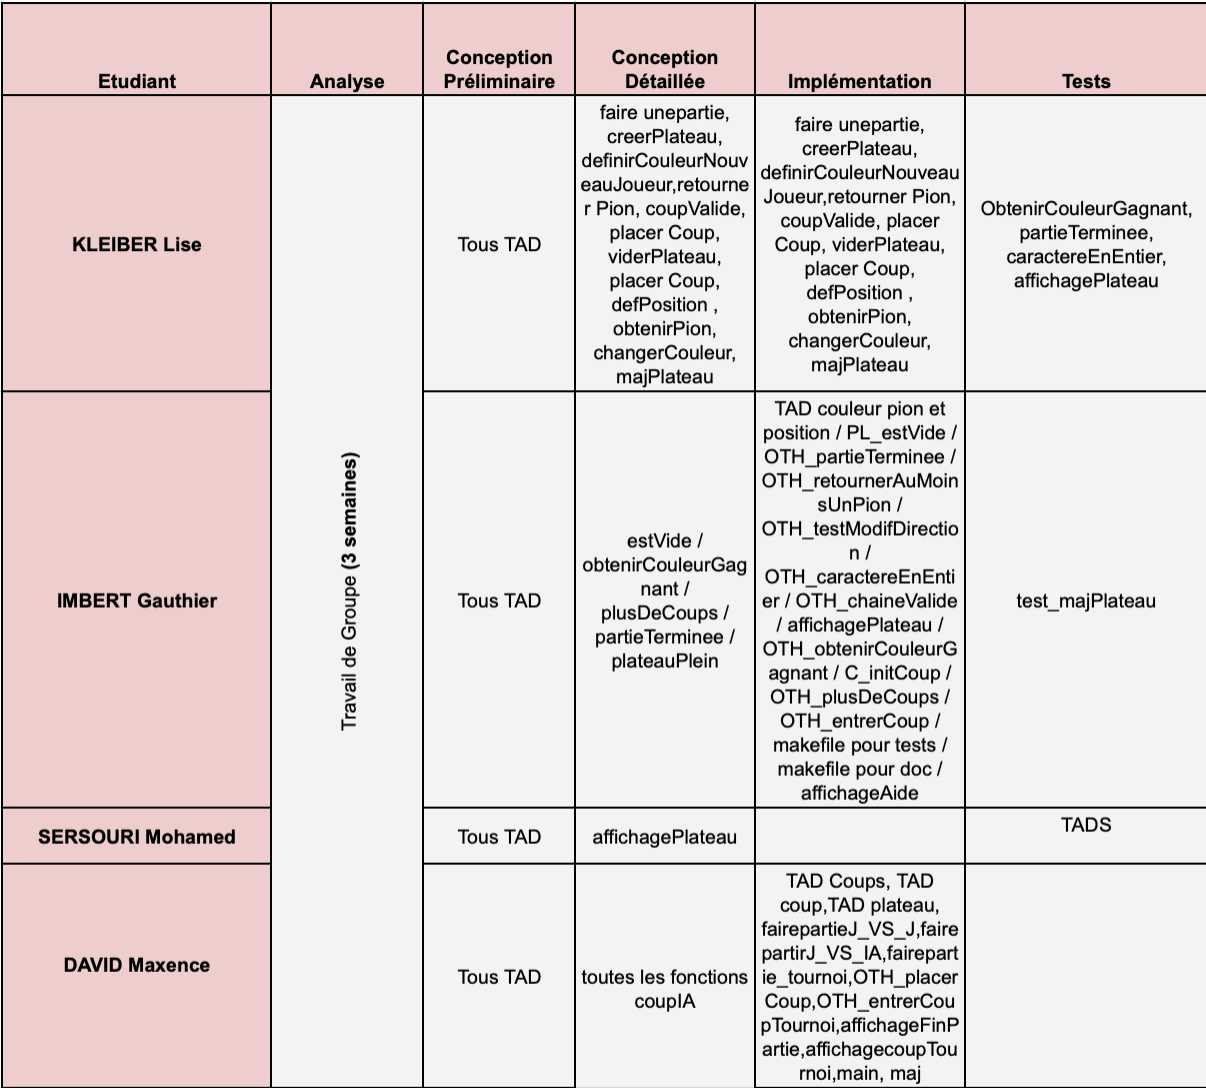
\includegraphics[scale=0.75]{travail.png}
\newpage
\subsection{Code en C : les .h}
\subsubsection{position.h}
\begin{lstlisting}
#ifndef __POSITION_OTHELLO__
#define __POSITION_OTHELLO__

typedef struct {
int positiony; /**< position y */
int positionx; /**< position x*/
}PO_Position;

PO_Position PO_defPosition(int y, int x);

int PO_ObtenirX(PO_Position position);

int PO_ObtenirY(PO_Position position);

int PO_Egal(PO_Position pos1, PO_Position pos2);

#endif

\end{lstlisting}

\subsubsection{plateau.h}
\begin{lstlisting}*
#ifndef __PLATEAU_OTHELLO__
#define __PLATEAU_OTHELLO__

#include "couleur.h"
#include "position.h"
#include "pion.h"

#define HAUTEUR 8

#define LARGEUR 8

typedef PI_Pion PL_Plateau[LARGEUR][HAUTEUR];  

void PL_QuatrePionsDebut(PL_Plateau* plateau);

void PL_Initialiser_Plateau(PL_Plateau* plateau);

PI_Pion PL_ObtenirPion(PO_Position position, PL_Plateau plateau);

void PL_PoserPion(PI_Pion pion, PO_Position position, PL_Plateau* plateau);

int PL_estVide(PO_Position position, PL_Plateau plateau);

void PL_CopierPlateau(PL_Plateau* plateau,PL_Plateau plateau_a_copier);

#endif
\end{lstlisting}
\subsubsection{pion.h}
\begin{lstlisting}

typedef struct {
	CO_Couleur couleurPion; /**< couleur du pion*/
	int etatPion; /**< etat du pion : 0 = inactif, autre =actif*/
}PI_Pion;

PI_Pion PI_CreerPion(CO_Couleur couleur);

void PI_ChangerEtat(PI_Pion pion);

CO_Couleur PI_ObtenirCouleurPion(PI_Pion pion);

int PI_Egal(PI_Pion pion1, PI_Pion pion2);

#endif

\end{lstlisting}

\subsubsection{coups.h}
\begin{lstlisting}

#ifndef __COUPS_OTHELLO__
#define __COUPS_OTHELLO__

#include "pion.h"
#include "coup.h"

#define MAX 64

typedef struct  { 
C_Coup tabcoups[MAX]; /**< tableau de coup 64 max car le plateau fait 64 cases*/
int nbcoups; /**< nombre de coups dans le tableau */
}CS_Coups;

CS_Coups CS_InitCoups();

int CS_EstVide (CS_Coups coups);

void CS_AjouterCoup (CS_Coups* coups,C_Coup coup);

C_Coup CS_IemeCoup (CS_Coups coups,int i);

int CS_NbCoups (CS_Coups coups );

int CS_EstPresent (CS_Coups coups,C_Coup coup);

void CS_SupprimerCoup (CS_Coups* coups,int i);

CS_Coups CS_ObtenirCoupsPossible (PL_Plateau pl, CO_Couleur CouleurReference );


#endif

\end{lstlisting}


\subsubsection{coup.h}
\begin{lstlisting}

typedef struct {
PO_Position positionCoup; /**< position du coup sur le plateau*/
PI_Pion Pion; /**< pion a placer (sa couleur)*/
}C_Coup;

C_Coup C_InitCoup(PO_Position position, PI_Pion pion);

C_Coup C_PlacerCoup(PI_Pion pion, PO_Position positionCoup);

PO_Position C_Obtenir_Position_Coup(C_Coup Coup);

PI_Pion C_obtenirPionCoup(C_Coup coup);

CO_Couleur C_Obtenir_Couleur_Coup(C_Coup Coup);

int C_Coup_Valide(C_Coup leCoup, PL_Plateau lePlateau);

int C_Egale(C_Coup coup1, C_Coup coup2);

#endif

\end{lstlisting}


\subsubsection{couleur.h}
\begin{lstlisting}
#ifndef __COULEUR__
#define __COULEUR__

typedef enum {BLANC,NOIR} CO_Couleur;

CO_Couleur CO_Blanc();

CO_Couleur CO_Noir();

CO_Couleur CO_ChangerCouleur(CO_Couleur CouleurActuelle );

int CO_estNoir(CO_Couleur UneCouleur);

int CO_estBlanc(CO_Couleur UneCouleur);

#endif

\end{lstlisting}

\subsubsection{affichagePlateau.h}
\begin{lstlisting}
#ifndef __AFFICHAGE_PLATEAU__
#define __AFFICHAGE_PLATEAU__

#include "plateau.h"
#include "position.h"
#include "coup.h"
typedef void (*affichagePlateau)(PL_Plateau);
typedef PO_Position (*entrerCoup)(CO_Couleur);
typedef void (entrerCoupTournoi)(PO_Position*,int* );

void OTH_affichagePlateau(PL_Plateau plateau);

PO_Position OTH_entrerCoup(CO_Couleur couleurJoueurCourant);

void OTH_entrerCoupTournoi(PO_Position* position, int* booleen);

void affichageFinPartie (CO_Couleur couleur);

void affichageAide();

void affichagecoupTournoi(C_Coup coup , int booleen);
#endif
\end{lstlisting}
\subsubsection{caractereEnEntier.h}
\begin{lstlisting}
#ifndef __CARACTERE_EN_ENTIER__
#define __CARACTERE_EN_ENTIER__

int OTH_chaineValide(char* chaine);

void OTH_chaineEnEntiers(char* chaine, int* entier1, int* entier2);

#endif

\end{lstlisting}
\subsubsection{coupIA.h}
\begin{lstlisting}
#ifndef __COUP_IA__
#define __COUP_IA__

#include "coups.h"
#include "plateau.h"
#include "coup.h"
#include "couleur.h"
#include "majPlateau.h"
#include <math.h>
#include <stdlib.h>
#include <stdio.h>

void IA_CoupIA(PL_Plateau pl,CO_Couleur CouleurReference,C_Coup* Resultat, int* estPossible);

int IA_scoreDUnCoup (C_Coup coup, PL_Plateau pl, CO_Couleur CouleurReference, int profondeur,int alpha , int beta  );

int IA_Alpha_Beta (PL_Plateau pl, CO_Couleur CouleurReference,CO_Couleur CouleurActuel, int profondeur,int alpha , int beta  );

int IA_Evalue (PL_Plateau pl, CO_Couleur CouleurReference );

#endif
\end{lstlisting}

\subsubsection{faireUnePartie.h}
\begin{lstlisting}
#ifndef __FAIRE_UNE_PARTIE__
#define __FAIRE_UNE_PARTIE__

#include <stdio.h>
#include "plateau.h"
#include "coup.h"
#include "couleur.h"
#include "caractereEnEntier.h"
#include "placerCoup.h"
#include "coupIA.h"

CO_Couleur OTH_faireUnePartie_J_VS_J();

CO_Couleur OTH_faireUnePartie_J_VS_IA(CO_Couleur couleurJoueurHumain);

CO_Couleur OTH_Tournoi(CO_Couleur CouleurJoueur);

#endif

\end{lstlisting}
\subsubsection{majPlateau.h}
\begin{lstlisting}
#ifndef __MAJ_Plateau__
#define __MAJ_Plateau__

#include "position.h"
#include "coup.h"
#include "plateau.h"
#include "placerCoup.h"
#include "position.h"
#include "pion.h"
#include <stdio.h>
#include <stdlib.h>
#include "couleur.h"

void OTH_majPlateau(PL_Plateau *lePlateau, C_Coup leCoup);

void OTH_retournerPion(PL_Plateau *lePlateau, PO_Position positionDuPion);

void maj (PL_Plateau* plateau,C_Coup coup);

#endif

\end{lstlisting}

\subsubsection{obtenirCouleurGagnant.h}
\begin{lstlisting}

#ifndef __OBTENIR_COULEUR_GAGNANT__
#define __OBTENIR_COULEUR_GAGNANT__

#include "couleur.h" 
#include "plateau.h"

void OTH_obtenirCouleurGagnant(PL_Plateau plateau, int* ilYaUnGagnant, CO_Couleur* couleurGagnant);

#endif
\end{lstlisting}
\subsubsection{partieTerminee.h}
\begin{lstlisting}

#ifndef __PARTIE_TERMINEE__
#define __PARTIE_TERMINEE__

#include "couleur.h"
#include "plateau.h"

int OTH_plateauPlein(PL_Plateau plateau);

int OTH_plusDeCoups(PL_Plateau plateau, CO_Couleur couleurJoueurCourant);

int OTH_partieTerminee(PL_Plateau plateau, CO_Couleur couleurJoueurCourant,CO_Couleur couleurAutreJoueur);

#endif
\end{lstlisting}

\newpage
\section{Code C}

\lstset{
    language=C,
    extendedchars=true,
    literate={à}{{\`a}}1 {é}{{\'e}}1 {è}{{\`e}}1 {ù}{{\`u'}}1 {î}{{\^i}}1 {ê}{{\^e}}1 {É}{{\'E}}1}
% src
\subsection{src}

\subsubsection{Position.c}
\lstinputlisting{../programme/src/position.c}
\vline

\subsubsection{Coup.c}
\lstinputlisting{../programme/src/coup.c}
\vline

\subsubsection{Coups.c}
\lstinputlisting{../programme/src/coups.c}
\vline

\subsubsection{Pion.c}
\lstinputlisting{../programme/src/pion.c}
\vline

\subsubsection{Couleur.c}
\lstinputlisting{../programme/src/couleur.c}
\vline

\subsubsection{Plateau.c}
\lstinputlisting{../programme/src/plateau.c}
\vline

\subsubsection{affichagePlateau.c}
\lstinputlisting{../programme/src/affichagePlateau.c}
\vline

\subsubsection{caractereEnEntier.c}
\lstinputlisting{../programme/src/caractereEnEntier.c}
\vline

\subsubsection{faireUnePartie.c}
\lstinputlisting{../programme/src/faireUnePartie.c}
\vline

\subsubsection{main.c}
\lstinputlisting{../programme/src/main.c}
\vline

\subsubsection{coupIA.c}
\lstinputlisting{../programme/src/coupIA.c}
\vline

\subsubsection{placerCoup.c}
\lstinputlisting{../programme/src/placerCoup.c}
\vline

\subsubsection{majPlateau.c}
\lstinputlisting{../programme/src/majPlateau.c}
\vline

\subsubsection{obtenirCouleurGagnant.c}
\lstinputlisting{../programme/src/obtenirCouleurGagnant.c}
\vline

\subsubsection{partieTerminee.c}
\lstinputlisting{../programme/src/partieTerminee.c}
\vline

% test

\subsection{Test}

\subsubsection{test-affichagePlateau.c}
\lstinputlisting{../programme/tests/srctest/test_affichagePlateau.c}
\vline

\subsubsection{test-caractereEnEntier.c}
\lstinputlisting{../programme/tests/srctest/test_caractereEnEntier.c}
\vline

\subsubsection{test-majPlateau.c}
\lstinputlisting{../programme/tests/srctest/test_majPlateau.c}
\vline

\subsubsection{test-obtenirCouleurGagnant.c}
\lstinputlisting{../programme/tests/srctest/test_obtenirCouleurGagnant.c}
\vline

\subsubsection{test-partieTerminee.c}
\lstinputlisting{../programme/tests/srctest/test_partieTerminee.c}
\vline

\subsubsection{testCouleur.c}
\lstinputlisting{../programme/tests/srctest/testCouleur.c}
\vline

\subsubsection{testCoup.c}
\lstinputlisting{../programme/tests/srctest/testCoup.c}
\vline

\subsubsection{testCoups.c}
\lstinputlisting{../programme/tests/srctest/testCoups.c}
\vline

\subsubsection{testPion.c}
\lstinputlisting{../programme/tests/srctest/testPion.c}
\vline

\subsubsection{testPlateau.c}
\lstinputlisting{../programme/tests/srctest/testPlateau.c}
\vline

\subsubsection{testPosition.c}
\lstinputlisting{../programme/tests/srctest/testPosition.c}
\vline






%\chapter{Analyse descendante}

%\begin{figure}[h]
%\centering
%\caption{Analyse descendante du projet}
%\rotatebox{270}{\includegraphics[scale=0.3]{analyse_descendante.png}}
%\end{figure}


%\input{ConceptionPreliminaire.tex}

%\input{ConceptionDetaillee.tex}

%\input{CahierDeSuivi}
\newpage


%\input{CodeC.tex}
\end{document}